% Autor: Leonhard Segger, Alexander Neuwirth
% Datum: 2017-10-30
\documentclass[
	% Papierformat
	a4paper,
	% Schriftgröße (beliebige Größen mit „fontsize=Xpt“)
	12pt,
	% Schreibt die Papiergröße korrekt ins Ausgabedokument
	pagesize,
	% Sprache für z.B. Babel
	ngerman
]{scrartcl}

% Achtung: Die Reihenfolge der Pakete kann (leider) wichtig sein!
% Insbesondere sollten (so wie hier) babel, fontenc und inputenc (in dieser
% Reihenfolge) als Erstes und hyperref und cleveref (Reihenfolge auch hier
% beachten) als Letztes geladen werden!

% Silbentrennung etc.; Sprache wird durch Option bei \documentclass festgelegt
\usepackage{babel}
% Verwendung der Zeichentabelle T1 (Sonderzeichen etc.)
\usepackage[T1]{fontenc}
% Legt die Zeichenkodierung der Eingabedatei fest, z.B. UTF-8
\usepackage[utf8]{inputenc}
% Schriftart
\usepackage{lmodern}
% Zusätzliche Sonderzeichen
\usepackage{textcomp}

% Mathepaket (intlimits: Grenzen über/unter Integralzeichen)
\usepackage[intlimits]{amsmath}
% Ermöglicht die Nutzung von \SI{Zahl}{Einheit} u.a.
\usepackage{siunitx}
% Zum flexiblen Einbinden von Grafiken (\includegraphics)
\usepackage{graphicx}
% Abbildungen im Fließtext
\usepackage{wrapfig}
% Abbildungen nebeneinander (subfigure, subtable)
\usepackage{subcaption}
% Funktionen für Anführungszeichen
\usepackage{csquotes}
\MakeOuterQuote{"}
% Zitieren, Bibliographie
\usepackage{biblatex}


% Zur Darstellung von Webadressen
\usepackage{url}
%chemische Formeln
\usepackage[version=4]{mhchem}
% siunitx: Deutsche Ausgabe, Messfehler getrennt mit ± ausgeben
\usepackage{floatrow}
\floatsetup[table]{capposition=top}
\usepackage{float}
% Verlinkt Textstellen im PDF-Dokument
\usepackage[unicode]{hyperref}
% "Schlaue" Referenzen (nach hyperref laden!)
\usepackage{cleveref}
\sisetup{
	locale=DE,
	separate-uncertainty
}
\bibliography{14Mo_W2_28-05-2018_References}

\begin{document}
	
	\begin{titlepage}
		\centering
		{\scshape\LARGE Versuchsbericht zu \par}
		\vspace{1cm}
		{\scshape\huge W2 - Adiabatenexponent $c_p/c_v$ von Gasen \par} %mit c_p/c_v oder ohne?
		\vspace{2.5cm}
		{\LARGE Gruppe 14Mo \par}
		\vspace{0.5cm}
		
		{\large Alexander Neuwirth (E-Mail: a\_neuw01@wwu.de) \par}
		{\large Leonhard Segger (E-Mail: l\_segg03@uni-muenster.de) \par}
		\vfill
		
		durchgeführt am 28.05.2018\par
		betreut von\par
		{\large Pascal Grenz}
		
		\vfill
		
		{\large \today\par}
	\end{titlepage}
	\tableofcontents
	\newpage

	%TODO mehr TODO in Default	

	\section{Kurzfassung}
	%TODO Hypothese	und deren Ergebnis, wenn Hypothese ist, dass nur Theorie erfüllt, sagen: Erwartung: Theorie aus einführung (mit reflink) erfüllt
	%TODO Ergebnisse, auch Zahlen, mindestens wenn's halbwegs Sinn ergibt
	%TODO Was wurde gemacht
	%TODO manche leute wollen Passiv oder "man", manche nicht
	
	
	\section{Methoden} \label{sec_Methoden}
	%TODO Bilder von der Website klauen
	Es wurden zwei verschiedene Experimente zur Bestimmung des Adiabatenexponenten durchgeführt:
	\subsection{Rüchardt-Flammersfeld}
	
	\begin{figure}[H]
		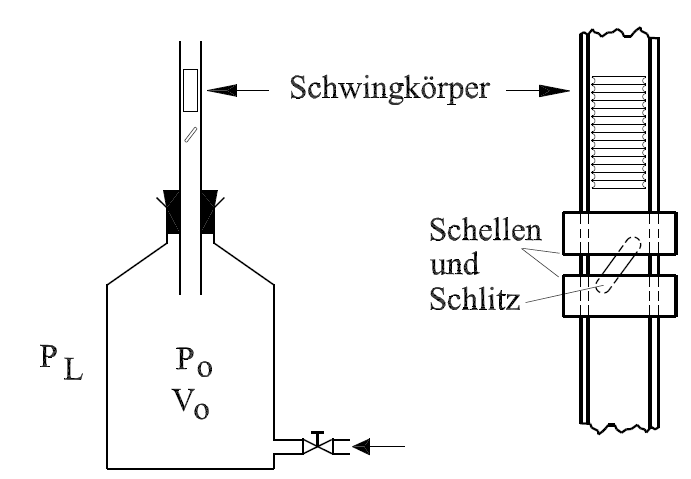
\includegraphics[width=0.4\textwidth]{flammer}
		\centering
		\caption{Experiment nach Rüchardt und Flammersfeld. \cite{abbildungen}}
		\label{aufbau_flammer}
		\centering
	\end{figure} 

	Das Experiment wurde wie in \cref{aufbau_flammer} aufgebaut.
	Ein Gas strömte in eine Flasche, auf die ein Glasrohr aufgesetzt war.
	Dieses Glasrohr war mit einem Schlitz versehen, dessen wirksame Lochgröße durch zwei verschiebbare Schellen begrenzt wurde.
	Nun wurde ein Schwingkörper in das Glasrohr gebracht und der Gasstrom so eingestellt, dass der Schwingkörper eine symmetrische Schwingung um das Loch ausführt.
	Für die Gase Luft, Argon und Kohlenstoffdioxid wurde die Zeit für je 100 Schwingungen und sechs verschiedene Abstände der Schellen gemessen.
	Zwischen dem Wechseln des Gases wurde das Glasrohr und der Schwingkörper mit einem Lederlappen gereinigt, um Abweichungen durch elektrische Ladungen zu minimieren.
	Außerdem wurde die Masse des Schwingkörpers bestimmt.
	
	\subsection{Clément-Desormes}
	
	\begin{figure}[H]
		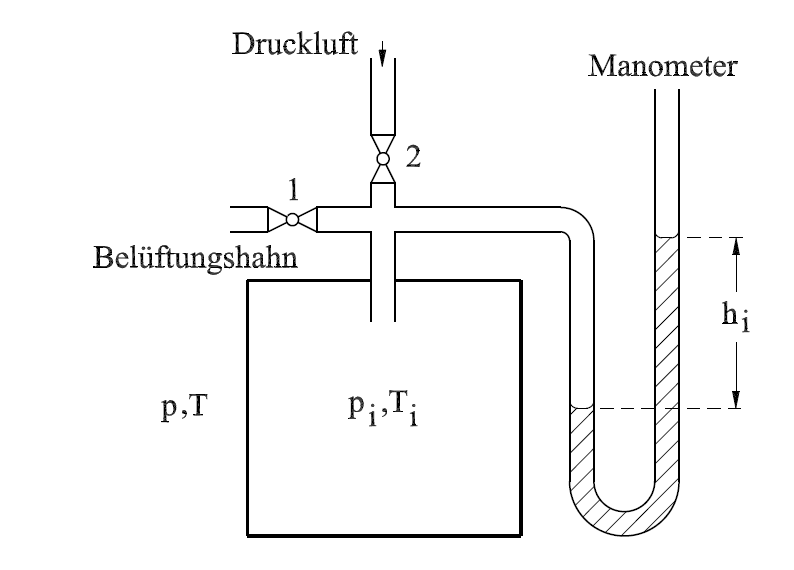
\includegraphics[width=0.4\textwidth]{clement}
		\centering
		\caption{Experiment nach Clément und Desormes. \cite{abbildungen}} %Clement hat apparently die Tochter seines Kollegen geheiratet und hieß dann Clement-Desormes, aber der Experimentname bezieht sich auf ihn und den Schwiegervater aka Kollegen.
		\label{aufbau_clement}
		\centering
	\end{figure} 
	
	Das Experiment wurde gemäß \cref{aufbau_clement} aufgebaut, wobei das Gasgefäß durch eine Plastiktonne realisiert wurde.
	Das Manometer war mit einer gefärbten Flüssigkeit gefüllt und die Druckluft durch einen Handblasebalg zugeführt.
	Belüftungshahn 1 wurde geschlossen und Druckluft durch den geöffneten Hahn 2 zugeführt.
	Dann wurde dieser auch geschlossen und gewartet, bis sich der Stand des Manometers nicht mehr änderte.
	Sobald dies der Fall war, wurde dieser gemessen und dann der Belüftungshahn so kurz geöffnet, dass der Druckausgleich mit der Umgebung gerade möglich war.
	Erneut wurde gewartet, bis sich das Manometer nicht mehr änderte und dann dieses abgelesen.
	Dies wurde fünf mal durchgeführt.
	
	\section{Ergebnisse und Diskussion}
	%TODO Unsicherheiten
	

	% \subsection{Beobachtung}
	%TODO Einflüsse von veränderten Parametern auf Messung
	\subsection{Beobachtungen und Datenanalyse}
	\subsubsection{Unsicherheiten} %TODO GGF IN DATENANYLSY
	Die Unsicherheiten wurden gemäß GUM ermittelt. 
	Außerdem wurde für Unsicherheitsrechnungen die Python Bibliothek "uncertainties" verwendet.
	\begin{description}
		\item[Waage:] Die Waage zeigt das Gewicht mit einer Nachkommastelle an, woraus eine Unsicherheit von \SI{0,03}{g} folgt (rechteckige WDF).
		\item[Stoppuhr:] Die Zeit wurde in Sekunden mit zwei Nachkommastellen gemessen. Folglich beträgt die Unsicherheit \SI{0,003}{s} (rechteckige WDF), jedoch hat die Reaktionszeit einen größeren Einfluss, weshalb eine Unsicherheit von \SI{0,1}{s} angenommen wird.
		\item[Messschieber:] Die Unsicherheit des Messschiebers wurde auf \SI{0,06}{mm}  abgeschätzt (dreieckige WDF).
		\item[Maßstäbe:]  Analoge Messung zum Messschieber, wobei die Unsicherheit \SI{0,04}{cm} beträgt.
		\item[Schwingungszählung:] Beim Zählen der 100 Schwingungen wird von maximal einer Schwingung zu viel bzw. zu wenig ausgegangen, sodass die Unsicherheit \SI{0,6}{} beträgt (rechteckige WDF).
		\item[Luftdruck:] Der Umgebungsdruck wurde anhand eines Barometers mit einer Unsicherheit von \SI{0,4}{kPa} ermittelt.
		\item[Glasflasche:] Auf der Glasflasche war keine Unsicherheit angegeben. Außerdem war unklar, ob das Volumen des Stöpsels, der die Flasche mit dem Glasrohr verbunden hat, mit in die Angabe von $\SI{5450}{cm^3}$ eingegangen ist. Deshalb wurde die Unsicherheit des Volumens mit $\SI{30}{cm^3}$ abgeschätzt.
	\end{description}
	
	\subsubsection{Bestimmung von $\kappa$ nach Rüchardt-Flammersfeld}
	Es wurde, wie in \cref{sec_Methoden} beschrieben, die Zeit für 100 Schwingungen bei unterschiedlichen Abständen der Schellen gemessen.
	In \cref{fig_Rüc_Fla} sind die Schwingdauern von Luft, Argon und Kohlenstoffdioxid gegen den Abstand der Schellen aufgetragen. 
	Es wurde ein linearer York-Fit verwendet, da dieser auch die X-Fehler berücksichtigt.
	Aus den Y-Achsenabschnitten der Fit-Funktionen lassen sich die Schwingdauern für einen auf Null extrapolierten Wert des Schellenabstands bestimmen.
	Diese sind in \cref{tab_Rüc_Fla} aufgeführt.
	
	\begin{figure}[H]
		\includegraphics[width=1\textwidth]{Rüc_Fla}
		\centering
		\caption{Gemessene Schwingdauern in Abhängigkeit vom Abstand der Schellen.}
		\label{fig_Rüc_Fla}
		\centering
	\end{figure} 

	In der Einführung wurde folgende Formel zur Bestimmung es Adiabatenexponenten hergeleitet:
	\begin{equation}
	\kappa = \frac{4\pi^2mV_0}{p_0 A^2 T^2}
	\label{eq_Rüc_Fla_Kappa}
	\end{equation}
	\begin{equation}
	u(\kappa) = \kappa \sqrt{\left(\frac{u(m)}{m}\right)^2+\left(\frac{u(V_0)}{V_0}\right)^2+\left(\frac{u(p_0)}{p_0}\right)^2+\left(\frac{2u(T)}{T}\right)^2+\left(\frac{2u(A)}{A}\right)^2}
	\end{equation}
	
	Das Volumen $V_0$ setzt sich zusammen aus dem der Glasflasche $V_F$ = $\SI{5450+-30}{cm^3}$ und dem des Glasrohrs mit einem Radius $r$ = $\SI{0,798+-0,003}{cm}$ und einer Höhe zum Spalt $h$ = $\SI{10,05+-0.06}{cm}$.
	\begin{equation}
		V_0 = V_F + r^2 \pi h
	\end{equation}
	Somit betragen:
	\begin{itemize}
		\item Volumen $V_0 = \SI{5470+-30}{cm^3}$.
		\item Fläche $A = r^2\pi = \SI{1,998+-0,015}{cm^2}$
		\item Masse $m = \SI{7,2+-0,03}{g}$ (Messung)
		\item Umgebungsdruck $p_\text{L}=\SI{101,2+-0,4}{kPa}$ (Messung)
		\item Innendruck $p_0 = p_\text{L} + \frac{m\cdot g}{A} = \SI{101,5+-0,4}{kPa}$ 
	\end{itemize}
	In \cref{tab_Rüc_Fla} sind die berechneten Adiabatenkoeffizienten zu den jeweiligen Schwingdauern aufgelistet.
	
	\begin{table}[H]
		\centering
		\begin{tabular}{ c | c | c | c}
			&Luft & Argon  & Kohlenstoffdioxid\\ \hline
			Schwingungsdauer $T$ in s&\SI{0,533+-0,003}{}&\SI{0,506+-0,003}{} & \SI{0,557+-0,003}{}\\
			Adiabatenkoeffizient $\kappa$ &\SI{1,351+-0,028}{}&\SI{1,499+-0,031}{}&\SI{1,237+-0,025}{}\\
		\end{tabular}
		\caption{Extrapolierte Schwingdauern sowie resultierende Adiabatenkoeffizienten.}
		\label{tab_Rüc_Fla} 
	\end{table}
	
	
	
	\subsubsection{Bestimmung von $\kappa$ nach Clément-Desormes}
	In der Einführung wurde folgende Formel zur Bestimmung des Adiabatenexponenten hergeleitet:
	\begin{equation}
		\kappa = \frac{h_1}{h_1-h_3}
		\label{eq_Cle_Des_Kappa}
	\end{equation}
	\begin{equation}	
		u(\kappa) = \kappa^2\cdot \sqrt{\left(\frac{h_3}{h_1}\right)^2+1} \cdot \frac{u(h)}{h_1}
	\end{equation}
	Dabei ist $h_1$ die Höhe der Flüssigkeitssäule im Manometer nach der Erhöhung des Drucks im Gefäß und dessen folgender Temperaturausgleich mit der Umgebung. 
	$h_3$ ist die Höhe, die sich ergibt, wenn man den Druck im Gefäß an den der Umgebung anpasst und sich, unter Druckänderung, ein (adiabatischer) Temperaturgleichgewicht einstellt.
	
	In \cref{tab_Manometer} sind die Messwerte und die Adiabatenkoeffizienten aufgeführt. Es folgt ein Mittelwert für $\kappa_\text{Luft}$ von \SI{1,355+-0,004}{}.
	\begin{table}[H]
		\centering
		\begin{tabular}{ c | c | c }
			$h_1$ in \SI{}{cm} & $h_3$ in \SI{}{cm}  & $\kappa_\text{Luft}$\\ \hline
			\SI{16,64+-0,06}{}&\SI{4,35+-0,06}{} & \SI{1,354+-0,007}{}\\
			\SI{20,63+-0,06}{}&\SI{5,52+-0,06}{}& \SI{1,365+-0,006}{}\\
			\SI{25,34+-0,06}{}&\SI{6,72+-0,06}{}& \SI{1,361+-0,005}{}\\
			\SI{36,7+-0,06}{}&\SI{9,41+-0,06}{}& \SI{1,345+-0,003}{}\\
			\SI{10,98+-0,06}{}&\SI{2,84+-0,06}{}& \SI{1,349+-0,01}{}\\
		\end{tabular}
		\caption{Gemessene Höhe der Flüssigkeitssäule im Manometer und nach \cref{eq_Cle_Des_Kappa} berechnete Adiabtenexponenten $\kappa_\text{Luft}$ von Luft.}
		\label{tab_Manometer} 
	\end{table}
	\subsection{Diskussion}
	%TODO Bezug/Nutzten oder sonst was
	%TODO auch hier die Hypothese wiederholen
	%TODO keine Messwerte hier, nach manchen Menschen, zumindest "direkt" erstellte Diagramme net hier, auch wenn Lesbarkeit-bla
	
	Es wurde erwartet, dass, wenn man gemäß \cref{eq_Freiheit} aus den Adiabatenexponenten, die sich aus den Messungen ergaben, die Freiheitsgrade des jeweiligen Gases bestimmt, sich innerhalb der Messunsicherheiten eine natürliche Zahl ergibt, die mit den in der Regel bei Raumtemperatur angeregten Freiheitsgraden, die in der Einführung gegeben waren, übereinstimmt. %langer Satz=>unschön, aber w/e
	Außerdem wurde angenommen, dass die hier die Freiheitsgrade im Fall von Luft bei der Messung durch das Experiment nach Rüchardt-Flammersfeld innerhalb der Unsicherheiten mit denen durch das Experiment nach Clément-Desormes übereinstimmen.
	In der Einführung wurde folgende Formel zum Zusammenhang zwischen Adiabatenexponent und angeregten Freiheitsgraden angegeben:
	\begin{equation}
		\kappa = \frac{f+2}{f}
	\end{equation}
	Oder umgeformt:
	\begin{equation}
		f = \frac{2}{\kappa -1}
		\label{eq_Freiheit}
	\end{equation}
	\begin{equation}
	u(f) = \frac{2}{(\kappa -1)^2} u(\kappa) 
	\end{equation}
	Die so berechneten angeregten Freiheitsgrade sind in \cref{tab_Freiheit} angegeben.
	
	\begin{table}[H]
		\centering
		\begin{tabular}{ c | c | c | c }
			Gas & Rüchardt-Flammersfeld  & Clément-Desormes & Erwartung \\ \hline
			Luft & \SI{5,698 \pm 0,455}{} & \SI{5,634 \pm 0,063}{} & 5\\
			Argon & \SI{4,008 \pm 0,249}{} & - & 3\\
			Kohlenstoffdioxid & \SI{8,439 \pm 0,890}{} & - & 5\\
		\end{tabular}
		\caption{Experimentell bestimmte angeregte Freiheitsgrade von Luft, Argon und Kohlenstoffdioxid nach Rüchardt-Flammersfeld und nach Clément-Desormes sowie die nach der Einführung erwarteten angeregten Freiheitsgrade.}
		\label{tab_Freiheit}
	
	Luft besteht zum größten Teil aus Stickstoff und Sauerstoff, was beides zweiatomige Gase sind, weshalb gemäß der Einführung fünf angeregte Freiheitsgrade zu erwarten sind.
	Argon ist ein einatomiges Gas. %muss ich das belegen?
	Daher sind drei Freiheitsgrade zu erwarten.
	Kohlenstoffdioxid liegt als dreiatomiges, gestrecktes Molekül vor.
	Also erwartet man fünf Freiheitsgrade
	\end{table}
	
	%TODO Fit für Null extrapolier for Argon gf. fraglich
	%TODO Luft net optimal
	%TODO Nix Paralexen frei...
	%TODO Plastictopf ist (bissle) dehnbar /= adiabatisch
	%TODO Prüfen des Volumens Glasflasche
	%TODO check Flasche nur ein Gas
	
	\section{Schlussfolgerung}
	%TODO Rückgriff auf Hypothese und drittes Nennen dieser
	
	%TODO Quellen zitieren, Websiten mit Zugriffsdatum
	%TODO Verweise auf das Laborbuch (sind erlaubt)
	%TODO Tabelle + Bilder mit Beschriftung
	\printbibliography
\end{document}
